

\iffalse
    \title{Assignment}
    \author{EE24BTECH11028}
    \section{me}
    \chapter{2024}
  \fi
\item A rigid massless tetrahedron is placed such that vertex $O$ is at the origin and the other three vertices $a$,$B$, and $C$ lie on the coordinate axes as shown in the figure.The body is acted on by three point loads, of which one is acting at $A$ along $x$-axis and another at point $B$ along $y$-axis. For the body to be in equilibrium, the third point load acting at point $o$ must be\\\\
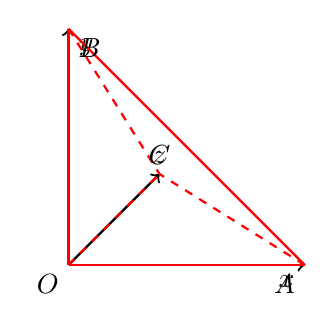
\begin{tikzpicture}
  % Axes
  \draw[->, thick] (0,0,0) -- (3,0,0) node[anchor=north east] {$x$};
  \draw[->, thick] (0,0,0) -- (0,3,0) node[anchor=north west] {$y$};
  \draw[->, thick] (0,0,0) -- (0,0,-3) node[anchor=south] {$z$};
  
  % Points
  \coordinate (O) at (0,0,0);
  \coordinate (A) at (3,0,0);
  \coordinate (B) at (0,3,0);
  \coordinate (C) at (0,0,-3);
  
  % Triangle edges
  \draw[thick, red] (O) -- (A);
  \draw[thick, red] (O) -- (B);
  \draw[thick, red,dashed] (O) -- (C);
  \draw[thick, red] (A) -- (B);
  \draw[thick, red,dashed] (B) -- (C);
  \draw[thick, red, dashed] (A) -- (C);
  
  % Labels
  \node[anchor=north east] at (A) {$A$};
  \node[anchor=north west] at (B) {$B$};
  \node[anchor=south] at (C) {$C$};
  \node[anchor=north east] at (O) {$O$};
\end{tikzpicture}\\
\begin{enumerate}
    \item along $z$-axis\\
    \item in $x-y$ plane but not along $x$ or $y$ axis\\
    \item in $y-z$ plane but not along $y$ or $z$ axis\\
    \item in $z-x$ plane but not along $z$ or $x$ axis
\end{enumerate}
\item The phases present in pearlite are\\
\begin{enumerate}
    \item austenite and ferrite\\
    \item cementite and austenite\\
    \item ferrite and cementite\\
    \item martensite and ferrite
\end{enumerate}
\item The "Earing" phenomenon in metal forming is associated with\\
\begin{enumerate}
    \item deep drawing\\
    \item rolling\\
    \item extrusion\\
    \item forging
\end{enumerate}
\item The grinding wheel used to provide the best surface finish is\\
\begin{enumerate}
   \item $A36L5V$\\
    \item $A54L5V$\\
    \item $60L5V$\\
   \item $80L5V$
\end{enumerate}
\item The allowance provided to a pattern for easy withdrawal from a sand mold is\\
\begin{enumerate}
    \item finishing\\
    \item shrinkage allowance\\
    \item distortion allowance\\
    \item shake allowance   
\end{enumerate}
   \item The most suitable electrode material used for joining low alloy steels using Gas Metal Arc Welding $\brak{GMAW}$\\
 \begin{enumerate}
   \item copper\\
   \item cadmium\\
   \item low alloy steel\\
   \item tungsten
 \end{enumerate}
 \item The preparatory function in computer numerical controlled $\brak{CNC}$ machine programing are denoted by the alphabet\\
 \begin{enumerate}
     \item $G$\\
     \item $M$\\
     \item $P$\\
     \item $O$
 \end{enumerate}
 \item A set of job $U$,$V$,$W$,$X$,$Y$,$Z$ arrive at time $t=0$ to a production line consisting of two workstations in series. Each jo must be processed by both workstations in sequence $\brak{i.e., the first followed by the second}$. The process time $\brak{in minutes}$ for each job on each workstation in the production line are given below.\\

 The sequence in which the jobs must be processed by the production line if the total makespan of production is to be minimized is\\
\begin{table}[h!]
\centering
\begin{tabular}{|c|c|c|c|c|c|c|}
\hline
\textbf{Job} & \textbf{U} & \textbf{V} & \textbf{W} & \textbf{X} & \textbf{Y} & \textbf{Z} \\ \hline
Workstation 1 & 5 & 7 & 3 & 4 & 6 & 8 \\ \hline
Workstation 2 & 4 & 6 & 6 & 8 & 5 & 7 \\ \hline
\end{tabular}
\end{table}
 
\begin{enumerate}
    \item$W-X-Z-V-Y-U$\\
    \item$W-X-V-Z-Y-U$\\
    \item$W-X-Z-V-Y-X$\\
    \item$U-Y-V-Z-X-W$\\
\end{enumerate}
\item A queueing system has one single server workstation that admits an infinitely long queue. The rate of arrival of job to the queueing system follows the poisson distribution with a mean of $5$ jobs/hour. The service time of the server is exponentially distributed with a man of $6$ minutes. In steady state operatation of the queueing system, the probability that the server is not busy at any point in time is\\
\begin{enumerate}
    \item$0.20$\\
    \item$0.17$\\
    \item$0.50$\\
    \item$0.83$\\
\end{enumerate}
\item The matrix $\myvec{1 && a\\ 8 && 3}$ $\brak{where a > 0}$ has a negative if $a$ is greater than\\
\begin{enumerate}
    \item$\frac{3}{8}$\\
     \item$\frac{1}{8}$\\
      \item$\frac{1}{4}$\\
       \item$\frac{1}{5}$\\
\end{enumerate}
\item In the pipe network shown in the figure, all pipes have the same cross-section and
can be assumed to have the same friction factor. The pipes connecting points $W$, $N$,
and $S$ with point $J$ have an equal length $L$. The pipe connecting points $J$ and $E$ has a
length $10L$. The pressures at the ends $N$, $E$, and $S$ are equal. The flow rate in the pipe
connecting $W$ and $J$ is $Q$. Assume that the fluid flow is steady, incompressible, and
the pressure losses at the pipe entrance and junction are negligible. Consider the
following statements:\\
$I$ : The flow rate in pipe connecting $J$ and $E$ is $Q/21$.\\
$II$: The pressure difference between $J$ and $N$ is equal to the pressure difference
between $J$ and $E$.\\
Which one of the following options is CORRECT?\\

\begin{tikzpicture}
    % Draw the horizontal and vertical lines
    \draw[thick, ->] (-2, 0) -- (5, 0); % horizontal line (West to East)
    \draw[thick, ->] (0, -2) -- (0, 2); % vertical line (South to North)

    % Draw flow rate arrow and label
    \draw[thick, ->] (-3, 0) -- (-2.2, 0);
    \node at (-3.2, 0) {flow rate $Q$};

    % Mark intersection point J
    \fill (0, 0) circle (2pt);
    \node[above right] at (0, 0) {$J$};

    % Label points W, E, S, N
    \node[above] at (-2, 0) {$W$};
    \node[right] at (5, 0) {$E$};
    \node[below] at (0, -2) {$S$};
    \node[above] at (0, 2) {$N$};

    % Draw L segments with arrows
    \draw[<->] (-2, -0.4) -- (0, -0.4);
    \node[below] at (-0.75, 0) {$L$};

  %  \draw[<->] (4, 0) -- (5, 0);
  %\node[below] at (0.75, 0) {$L$};

    \draw[<->] (-0.5, 2) -- (-0.5, 0);
    \node[left] at (0, 0.75) {$L$};

    \draw[<->] (0.5, -2) -- (0.5, 0);
    \node[right] at (0, -0.75) {$L$};

    % Draw longer segment to the right with label
    \draw[<->] (5, 0.5) -- (0, 0.5);
    \node[above] at (3, 0) {$10L$};

    % "Not to scale" label box
    \node[draw, rectangle, minimum width=2cm, minimum height=0.8cm] at (3.5, -2) {not to scale};

\end{tikzpicture}



\begin{enumerate}
    \item $I$ is True and $I$I is False\\
    \item $I$ is False and $II$ is True\\
    \item Both $I$ and $II$ are True\\
     \item Both $I$ and $II$ are False\\
\end{enumerate}
\item A company orders gears in conditions identical to those considered in the economic
order quantity $\brak{EOQ}$ model in inventory control. The annual demand is $8000$ gears,
the cost per order is $300$ rupees, and the holding cost is $12$ rupees per month per gear.
The company uses an order size that is $25\%$ more than the optimal order quantity
determined by the EOQ model. The percentage change in the total cost of ordering
and holding inventory from that associated with the optimal order quantity is\\
\begin{enumerate}
\item $2.5$\\
\item $5$\\
\item $0$\\
\item $12.5$\\
\end{enumerate}
\item At the current basic feasible solution $\brak{bfs} v_{0} \brak{v_{0} \in R^{5}}$, the simplex method yields the following form of a linear programming problem in standard form.
minimize $z=-x_{1}-2x_{2}$\\
s.t      $x_{3}=2+2x_{1}-x_{2}$\\
         $x_{5}=3-x_{1}$\\
         $x_{1},x_{2},x_{3},x_{4},x_{5} \geq$
Here the objective function is written as a function of the non-basic variables. If the
simplex method moves to the adjacent bfs $v_{1} \brak{v_{1} \in R^{5}}$ that best improves the
objective function, which of the following represents the objective function at $v_{1}$,
assuming that the objective function is written in the same manner as above?\\
\begin{enumerate}
    \item$z=-4-5x_{1}+2x_{2}$\\
    \item$z=-3+x_{5}+2x_{2}$\\
    \item$z=-4-5x_{1}+2x_{4}$\\
    \item$z=-6-5x_{1}+2x_{3}$\\
\end{enumerate}
 
